\documentclass[12pt,ucs,hyperref={pdftext}]{beamer}
%\documentclass[12pt, a4paper]{article}
\mode<presentation>

\newif\ifpdf
\ifx\pdfoutput\undefined
\pdffalse % we are not running PDFLaTeX
\else
\pdfoutput=1 % we are running PDFLaTeX
\pdftrue
\fi
%\usetheme{Warsaw}
%\usetheme{Berkeley}
%\usetheme{PaloAlto}
\usetheme{Luebeck}
\usecolortheme[]{seagull}
%\usecolortheme[]{beaver}

%\usepackage{mathptmx}
%\usepackage{helvet}

\usepackage[utf8x]{inputenc}
\usepackage[english]{babel}
%\usepackage{german}
%\usepackage{longtable}
%\usepackage{tocbibind}
%\usepackage{makeidx}
%\usepackage{amsmath}
%\usepackage{amsfonts}
%\usepackage{amssymb}
%\usepackage{pdfsync}  % enable tex source and pdf output syncronicity
%\usepackage[all]{xy}
\usepackage{multicol}
%\usepackage{wrapfig}
\usepackage{listings}

\lstset{
	language=C++,
	basicstyle=\scriptsize, % print whole listing small
	keywordstyle=\color{blue},%\bfseries,
	% underlined bold black keywords
	identifierstyle=, % nothing happens
	commentstyle=\color{green}, % white comments
	%stringstyle=\ttfamily, % typewriter type for strings
	showstringspaces=false,
	%numbers=left, numberstyle=\tiny, stepnumber=1, numbersep=5pt,
	columns=flexible,% fixed
	breaklines=true
}

\hypersetup{
    pdftitle={Tool support for user testing of stereoscopic fatigue},
%    pdfsubject={Subject of the document}, % Subject
    pdfauthor={Gerhard Roethlin},              % Author
    pdfkeywords={master, fatigue testing software, stereo vision},       % Keywords
}

%\renewcommand{\labelitemi}{-}

\setcounter{tocdepth}{2}

\setbeamercovered{transparent}
\setbeamersize{description width=0.5cm}
\newlength{\columnleft}
\newlength{\columnright}
\setlength{\columnleft}{5cm}
\setlength{\columnright}{6cm}

%\titlegraphic{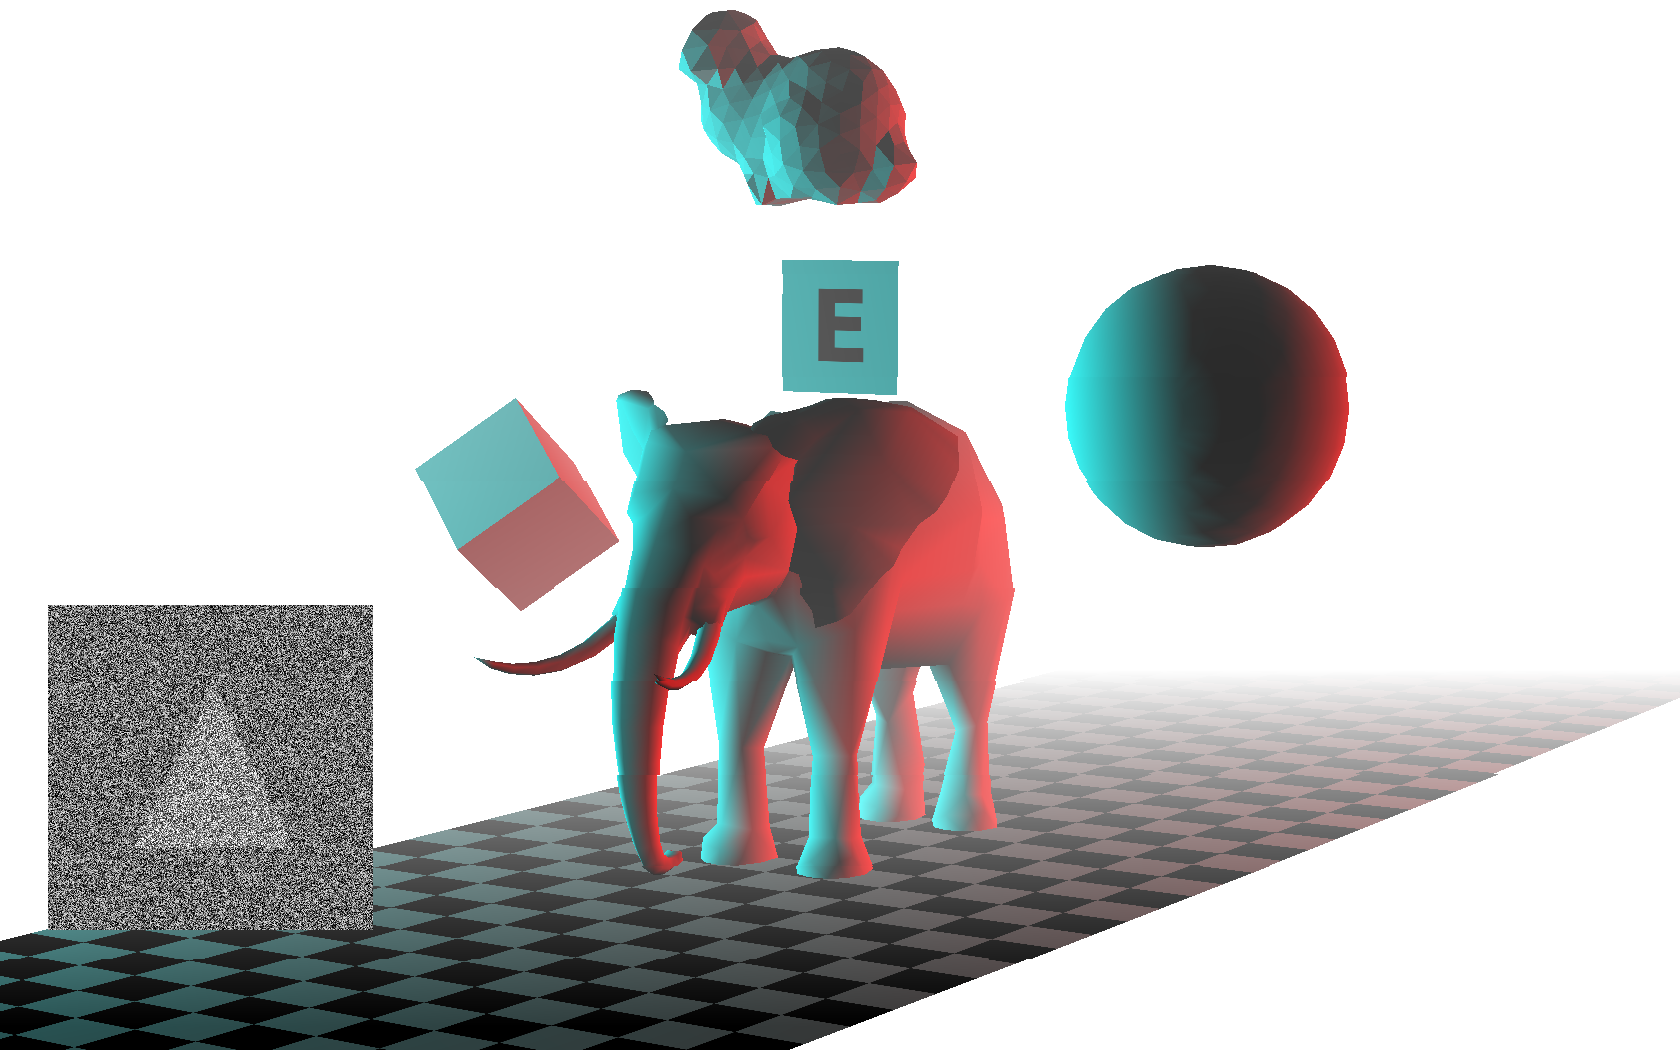
\includegraphics[width=7.5cm,clip,trim=0cm 6cm 0cm 2cm]{media/title.png}}
\title{ExaminationRoom}
\subtitle{Tool support for user testing of stereoscopic fatigue}
\author[gerhardr]{Gerhard R\"othlin {\tt\normalsize <gerhardr@student.ethz.ch>}}
\date{2008.07.07}

\begin{document}

\ifpdf
\DeclareGraphicsExtensions{.pdf, .jpg, .tif, .tiff, .png}
\else
\DeclareGraphicsExtensions{.eps, .jpg}
\fi

\begin{frame}

\titlepage
%\inserttitlegraphic
%\inserttitle
%\insertsubtitle
%\insertauthor
%\insertdate
%\insertinstitute

\end{frame}

%\logo{\includegraphics[width=1cm,alpha=0.5]{media/icon-mayan.png}}


\section{Introduction}

\subsection{Outline}
\begin{frame}{Outline}
\begin{multicols}{2}
\tableofcontents
\end{multicols}
\end{frame}


\subsection{Motivation}

\begin{frame}{Motivation}
\begin{columns}

\column{\columnleft}
%\includegraphics[width=4cm]{media/dollySurfaceTheory.jpg}

\column{\columnright}
\begin{itemize}%[<+-| alert@+>]%[<+->]
\item Todo
\item Todo
\end{itemize}

\end{columns}
\end{frame}

\section{Design}

\section{Implementation}

\subsection{Scene graph}

\subsection{Mechanics}

\subsection{User Interface}


\section{Demo}

\begin{frame}{Creation Demo}
A short demo of the test creation
\end{frame}

\begin{frame}{Test Demo}
A short demo of the testing
\end{frame}


\appendix


\subsection{End?}
\begin{frame}{End}
Questions?
\end{frame}

\subsection{Examples}



\end{document}
\end
